\documentclass[12pt, oneside]{article}
\usepackage[letterpaper, margin=1in, headsep=0.5in]{geometry}
\usepackage[english]{babel}
\usepackage[utf8]{inputenc}
\usepackage{amsmath}
\usepackage{amsfonts}
\usepackage{amssymb}
\usepackage{tikz}
\usetikzlibrary{quotes, angles}
\usepackage{graphicx}
%\usepackage{pgfplots}
%\pgfplotsset{width=10cm,compat=1.9}
%\usepgfplotslibrary{statistics}
%\usepackage{pgfplotstable}
%\usepackage{tkz-fct}
%\usepackage{venndiagram}

\usepackage{fancyhdr}
\pagestyle{fancy}
\fancyhf{}
\rhead{\thepage \\Name: \hspace{1.5in}.\\}
\lhead{BECA / Dr. Huson / Geometry 10th Grade\\* Unit 1b: Introduction to Geometry}

\renewcommand{\headrulewidth}{0pt}

\begin{document}
\subsubsection*{Do Now 1b.1: Drawing angles}
  \vspace{0.5cm}
  \begin{enumerate}
    \item Absolute value: Find the value of $|180-120|+|60-90|$. \vspace{2cm}

    \item Identify two rays in the given plane.\\[0.25in]
      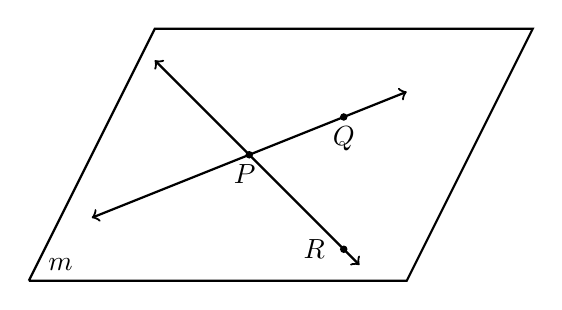
\begin{tikzpicture}[scale=0.8]
        \draw [thick](0,0) node[above right]{$\ m$} --(6,0)--(8,4)--(2,4)--(0,0);
        \draw [<->, thick] (1,1)--(6,3);
        \draw [fill] (3.5,2) circle [radius=0.05] node[below]{$P \ $};
        \draw [fill] (5,2.6) circle [radius=0.05] node[below]{$Q$};
        \draw [<->, thick] (2,3.5)--(5.25,.25);
        \draw [fill] (5,0.5) circle [radius=0.05] node[left]{$R \ $};
      \end{tikzpicture}
      \vspace{1cm}

    \item Given opposite rays $\overrightarrow{AB}$ and $\overrightarrow{AC}$, with $\overline{AB}=6$ cm. Draw a ray $\overrightarrow{AD}$ such that $m \angle BAD=60^\circ$ and $\overline{AD}=6$ cm.
    \vspace{7cm}
    \begin{center}
    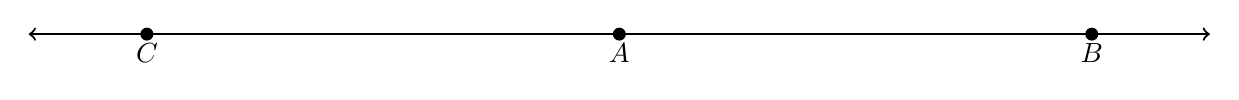
\begin{tikzpicture}[scale=1.5]
      \draw [->, thick] (0,0)--(-5,0);
      \draw [->, thick] (0,0)--(5,0);
      %\draw [->, thick] (0,0)--(-1.2,3);
      %\draw [fill] (-1,2.5) circle [radius=0.05] node[left ]{$B$};
      \draw [fill] (-4,0) circle [radius=0.05] node[below]{$C$};
      \draw [fill] (0,0) circle [radius=0.05] node[below]{$A$};
      \draw [fill] (4,0) circle [radius=0.05] node[below]{$B$};
    \end{tikzpicture}
    \end{center}

  \newpage
    \item Points that are all located on the same plane are $\rule{4cm}{0.15mm}$.

    \item Given collinear points $P, Q, R$ with $Q$ bisecting the line segment $\overline{PR}$. $PQ=x-2$ and $QR = \frac{1}{2} x+6$. Find the length of $\overline{PR}$.\\ \bigskip
    First label the drawing.
    \begin{flushright}
    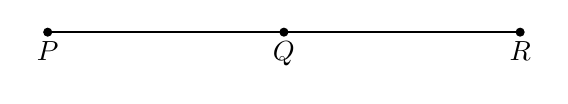
\begin{tikzpicture}
      \draw [-, thick] (0,0)--(6,0);
      \draw [fill] (0,0) circle [radius=0.05] node[below]{$P$};
      \draw [fill] (6,0) circle [radius=0.05] node[below]{$R$};
      \draw [fill] (3,0) circle [radius=0.05] node[below]{$Q$};
    \end{tikzpicture}
    \end{flushright}
    \vspace{1cm}
    \begin{enumerate}
      \item Write a geometric equation: \rule{4cm}{0.15mm} \hspace{1cm} \rule{4cm}{0.15mm}
      \vspace{.7cm}
      \item Substitute algebraic values: \rule{4cm}{0.15mm}
      \item Solve for $x$
      \vspace{4.5cm}
      %\begin{center} $x=$ \rule{1cm}{0.15mm} \end{center}
      \item Answer the question:
      \vspace{2.5cm}
      \item Check your answer
    \end{enumerate}

  \end{enumerate}

\newpage
\subsubsection*{Do Now 1b.4: Angle pairs} % Thursday Sept 26
  \vspace{0.5cm}
  \begin{enumerate}

    \item The sum of the measures of two supplementary angles equals $\rule{2cm}{0.15mm}$. \bigskip
    \item True or false: The angles making a linear pair are adjacent. $\rule{2cm}{0.15mm}$. \bigskip
    \item The sum of the measures of two complementary angles equals $\rule{2cm}{0.15mm}$. \bigskip
    \item True or false: The angles making a linear pair are complementary. $\rule{2cm}{0.15mm}$. \bigskip
    \item Two vertical angles are supplementary. What are their measures? $\rule{3cm}{0.15mm}$. \bigskip
    \item Sketch a linear pair. \vspace{3cm}

      \item Given the situation in the diagram, answer each question. \vspace{1cm}
        \begin{flushright}
        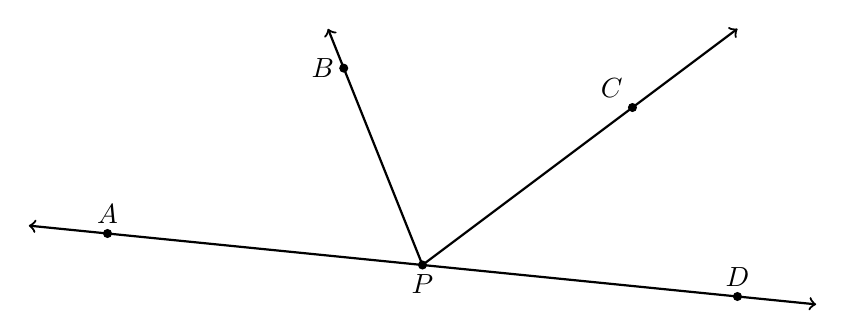
\begin{tikzpicture}[scale=1]
          \draw [->, thick] (0,0)--(4,3);
          \draw [<->, thick] (-5,.5)--(5,-.5);
          \draw [->, thick] (0,0)--(-1.2,3);
          \draw [fill] (-1,2.5) circle [radius=0.05] node[left ]{$B$};
          \draw [fill] (2.66666,2) circle [radius=0.05] node[above left ]{$C$};
          \draw [fill] (0,0) circle [radius=0.05] node[below]{$P$};
          \draw [fill] (4,-0.4) circle [radius=0.05] node[above]{$D$};
          \draw [fill] (-4,0.4) circle [radius=0.05] node[above]{$A$};
        \end{tikzpicture}
        \end{flushright}
      \begin{enumerate}
        \item True or false: $\overrightarrow{PA}$ and $\overrightarrow{PD}$ are opposite rays. $\rule{3cm}{0.15mm}$. \bigskip
        \item Name an angle adjacent to $\angle APB$. $\rule{3cm}{0.15mm}$. \bigskip
        \item True or false: $\angle APC$ and $\angle CPD$ are supplementary angles. $\rule{3cm}{0.15mm}$. \bigskip
        \item Name two angles that constitute a linear pair. $\rule{4cm}{0.15mm}$. \bigskip
      \end{enumerate}
  \newpage
            \item Given two supplementary angles: $m \angle 1 = 50$, $m \angle 2 = x$.\\ Find $x$. \vspace{2cm}
            \item Given two complementary angles: $m \angle 1 = x$, $m \angle 2 = 20$. Find $m \angle 1$. \vspace{2cm}

            \item Given two vertical angles: $m \angle 1 = 3x+10$, $m \angle 2 = 2x+25$. Find $m \angle 1$.\\
            First label the drawing.
            \begin{flushright}
            \begin{tikzpicture}[scale=.7]
              \draw [<->, thick] (0,-1.5)--(10,1.5);
              \draw [<->, thick] (2,3.5)--(7,-3.5);
              \node at (3,.4){1};
              \node at (6,-.6){2};
              %\draw [fill] (0,0) circle [radius=0.05] node[below]{$P$};
              %\draw [fill] (6,0) circle [radius=0.05] node[below]{$R$};
              %\draw [fill] (3,0) circle [radius=0.05] node[below]{$Q$};
            \end{tikzpicture}
            \end{flushright}
            %\vspace{.5cm}
            \begin{enumerate}
              \item Write a geometric equation: \rule{4cm}{0.15mm} \hspace{1cm} \rule{4cm}{0.15mm}
              \vspace{.7cm}
              \item Substitute algebraic values: \rule{4cm}{0.15mm}
              \item Solve for $x$
              \vspace{2cm}
              %\begin{center} $x=$ \rule{1cm}{0.15mm} \end{center}
              \item Answer the question:
              \vspace{2cm}
              \item Check your answer
            \end{enumerate}

  \end{enumerate}

  \newpage
\subsubsection*{Homework 1b.4: Angle pairs} % Thursday Sept 27
  \vspace{0.5cm}
  \begin{enumerate}

    \item True or false: The angles making a linear pair are supplementary. $\rule{2cm}{0.15mm}$. \bigskip
    \item The sum of the measures of two complementary angles equals $\rule{2cm}{0.15mm}$. \bigskip
    \item True or false: Vertical angles are congruent. $\rule{2cm}{0.15mm}$. \bigskip
    \item The sum of the measures of two supplementary angles equals $\rule{2cm}{0.15mm}$. \bigskip
    \item Two vertical angles are complementary. What are their measures? $\rule{3cm}{0.15mm}$. \bigskip
    \item Sketch a pair of vertical angles. \vspace{3cm}

      \item Given the situation in the diagram, answer each question. \vspace{1cm}
        \begin{flushright}
        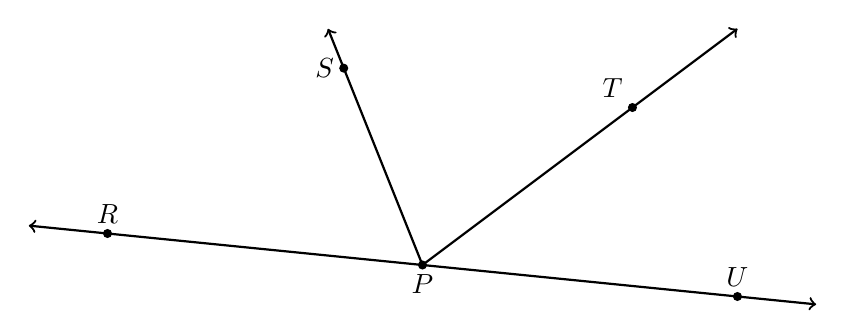
\begin{tikzpicture}[scale=1]
          \draw [->, thick] (0,0)--(4,3);
          \draw [<->, thick] (-5,.5)--(5,-.5);
          \draw [->, thick] (0,0)--(-1.2,3);
          \draw [fill] (-1,2.5) circle [radius=0.05] node[left ]{$S$};
          \draw [fill] (2.66666,2) circle [radius=0.05] node[above left ]{$T$};
          \draw [fill] (0,0) circle [radius=0.05] node[below]{$P$};
          \draw [fill] (4,-0.4) circle [radius=0.05] node[above]{$U$};
          \draw [fill] (-4,0.4) circle [radius=0.05] node[above]{$R$};
        \end{tikzpicture}
        \end{flushright}
      \begin{enumerate}
        \item True or false: $\overrightarrow{PR}$ and $\overrightarrow{PT}$ are opposite rays. $\rule{3cm}{0.15mm}$. \bigskip
        \item Name an angle adjacent to $\angle TPU$. $\rule{3cm}{0.15mm}$. \bigskip
        \item True or false: $\angle RPT$ and $\angle SPU$ are supplementary angles. $\rule{3cm}{0.15mm}$. \bigskip
        \item Name two angles that are adjacent. $\rule{4cm}{0.15mm}$. \bigskip
      \end{enumerate}

  \newpage
            \item Given two supplementary angles: $m \angle 1 = 135$, $m \angle 2 = x$.\\ Find $x$. \vspace{2cm}
            \item Given two complementary angles: $m \angle 1 = x$, $m \angle 2 = 75$. Find $m \angle 1$. \vspace{2cm}

            \item Given two vertical angles: $m \angle 1 = 7x+10$, $m \angle 2 = 2x+45$. Find $m \angle 1$.\\
            First label the drawing.
            \begin{flushright}
            \begin{tikzpicture}[scale=.7]
              \draw [<->, thick] (0,-1.5)--(10,1.5);
              \draw [<->, thick] (2,3.5)--(7,-3.5);
              \node at (3,.4){1};
              \node at (6,-.6){2};
              %\draw [fill] (0,0) circle [radius=0.05] node[below]{$P$};
              %\draw [fill] (6,0) circle [radius=0.05] node[below]{$R$};
              %\draw [fill] (3,0) circle [radius=0.05] node[below]{$Q$};
            \end{tikzpicture}
            \end{flushright}
            %\vspace{.5cm}
            \begin{enumerate}
              \item Write a geometric equation: \rule{4cm}{0.15mm} \hspace{1cm} \rule{4cm}{0.15mm}
              \vspace{.7cm}
              \item Substitute algebraic values: \rule{4cm}{0.15mm}
              \item Solve for $x$
              \vspace{2cm}
              %\begin{center} $x=$ \rule{1cm}{0.15mm} \end{center}
              \item Answer the question:
              \vspace{2cm}
              \item Check your answer
            \end{enumerate}
          \end{enumerate}

  \newpage
\subsubsection*{Do Now 1b.5: Angle pairs} % Friday Sept 28
  %\vspace{0.5cm}
  \begin{enumerate}
    \item The sum of the measures of two supplementary angles equals $\rule{2cm}{0.15mm}$. \bigskip
    \item The sum of the measures of two complementary angles equals $\rule{2cm}{0.15mm}$.
    \item Draw a pair of vertical angles: $\angle 1$, $\angle 2$. \vspace{2cm}
    \item Draw a linear pair of angles: $\angle ABC$, $\angle CBD$. \vspace{3cm}

    \item Given two perpendicular rays, $\overrightarrow{BA}$ and $\overrightarrow{BC}$, as shown. $m \angle ABD = 2x+10$, $m \angle DBC = x+5$. Find $m \angle DBC$.
    First label the drawing.
    \begin{flushright}
    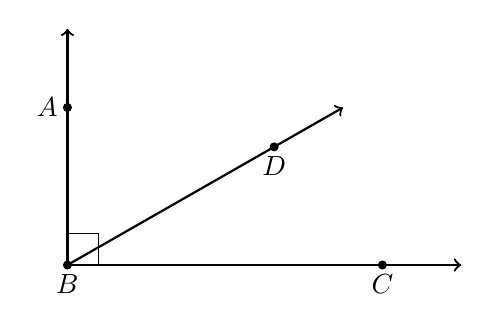
\begin{tikzpicture}[scale=1]
      \draw [<->, thick] (0,3)--(0,0)--(5,0);
      \draw [->, thick] (0,0)--(3.5, 2);
      \draw [-, thin] (0, 0.4)--(0.4, 0.4)--(0.4, 0);
      %\node at (3,.4){1};
      %\node at (6,-.6){2};
      \draw [fill] (0,0) circle [radius=0.05] node[below]{$B$};
      \draw [fill] (0,2) circle [radius=0.05] node[left]{$A$};
      \draw [fill] (4,0) circle [radius=0.05] node[below]{$C$};
      \draw [fill] (2.625, 1.5) circle [radius=0.05] node[below]{$D$};
    \end{tikzpicture}
    \end{flushright}
    %\vspace{.5cm}
    \begin{enumerate}
      \item Write a geometric equation: \rule{4cm}{0.15mm} \hspace{1cm} \rule{4cm}{0.15mm}
      \vspace{.5cm}
      \item Substitute algebraic values: \rule{4cm}{0.15mm}
      \item Solve for $x$
      \vspace{2cm}
      %\begin{center} $x=$ \rule{1cm}{0.15mm} \end{center}
      \item Answer the question:
      \vspace{1cm}
      \item Check your answer
    \end{enumerate}

  \end{enumerate}

\newpage
\subsubsection*{Do Now 1b.6: Angle pair practice} % Monday October 1
  %\vspace{0.5cm}
  \begin{enumerate}
    \item Given $m \angle A=60$, $m \angle B=20$, $m \angle 1=30$, $m \angle DEF=150$, $m \angle FEG=10$. \bigskip
    \begin{enumerate}
      \item Find a pair of complementary angles. \rule{3cm}{0.15mm} \hspace{1cm} \rule{3cm}{0.15mm} \bigskip
      \item Find a pair of supplementary angles. \rule{3cm}{0.15mm} \hspace{1cm} \rule{3cm}{0.15mm} \bigskip
      \item Spicy: Find a different pair of supplementary angles. \rule{3cm}{0.15mm} \hspace{1cm} \rule{3cm}{0.15mm}
    \end{enumerate}}

    \item Identify three points in the given plane.\\[0.25in]
      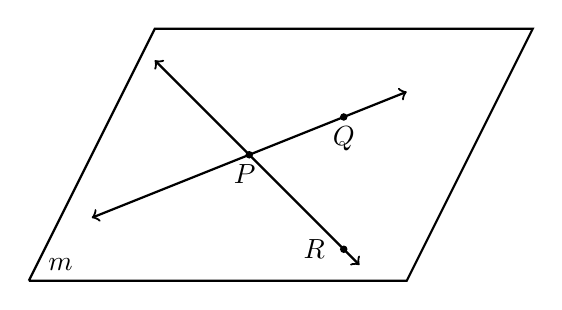
\begin{tikzpicture}[scale=0.8]
        \draw [thick](0,0) node[above right]{$\ m$} --(6,0)--(8,4)--(2,4)--(0,0);
        \draw [<->, thick] (1,1)--(6,3);
        \draw [fill] (3.5,2) circle [radius=0.05] node[below]{$P \ $};
        \draw [fill] (5,2.6) circle [radius=0.05] node[below]{$Q$};
        \draw [<->, thick] (2,3.5)--(5.25,.25);
        \draw [fill] (5,0.5) circle [radius=0.05] node[left]{$R \ $};
      \end{tikzpicture}
      \vspace{1cm}

      \item Given $\overleftrightarrow{QS}$ as shown on the number line. \\[10pt] %\vspace{1cm}
      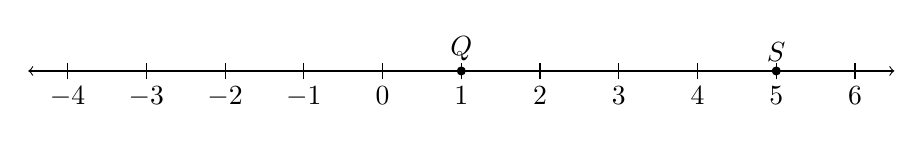
\begin{tikzpicture}
        \draw [<->] (-4.5,0)--(6.5,0);
        \foreach \x in {-4,...,6} %2 leading for diff!=1
          \draw[shift={(\x,0)},color=black] (0pt,-3pt) -- (0pt,3pt) node[below=5pt]  {$\x$};
          \draw [fill] (1,0) circle [radius=0.05] node[above] {$Q$};
          \draw [fill] (5,0) circle [radius=0.05] node[above] {$S$};
      \end{tikzpicture}
      \begin{enumerate}
        \item Mark the point $R$, the midpoint of $\overline{QS}$.
        \item The point $P$ is collinear with $\overleftrightarrow{QS}$ such that $Q$ is the midpoint of $\overleftrightarrow{PS}$. Mark $P$ on the line.
      \end{enumerate}}

      \item Points that are all located on the same plane are $\rule{4cm}{0.15mm}$.
      \item Find the value of $|1.5-4|-1$. \vspace{1cm}

      \item Given $\overline{ABC}$, $AC=5 \frac{1}{3}$, and $BC=1$.
      \begin{enumerate}
        \item Find ${AB}$.\\[0.75cm]
          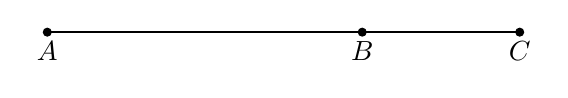
\begin{tikzpicture}
            \draw [-, thick] (1,0)--(7,0);
            \draw [fill] (1,0) circle [radius=0.05] node[below]{$A$};
            \draw [fill] (5,0) circle [radius=0.05] node[below]{$B$};
            \draw [fill] (7,0) circle [radius=0.05] node[below]{$C$};
          \end{tikzpicture} \bigskip
        \item The postulate used in this problem is the \rule{6cm}{0.15mm}.
      \end{enumerate}
      \newpage

      \item Given collinear points $P, Q, R$ with $Q$ bisecting the line segment $\overline{PR}$. $PQ=\frac{1}{2} x+4$ and $PR = 4x$. Find the length of $\overline{PR}$.\\ \bigskip
      First label the drawing.
      \begin{flushright}
      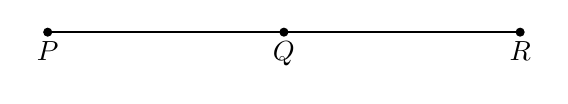
\begin{tikzpicture}
        \draw [-, thick] (0,0)--(6,0);
        \draw [fill] (0,0) circle [radius=0.05] node[below]{$P$};
        \draw [fill] (6,0) circle [radius=0.05] node[below]{$R$};
        \draw [fill] (3,0) circle [radius=0.05] node[below]{$Q$};
      \end{tikzpicture}
      \end{flushright}
      \vspace{1cm}
      \begin{enumerate}
        \item Write a geometric equation: \rule{4cm}{0.15mm} \hspace{1cm} \rule{4cm}{0.15mm}
        \vspace{.7cm}
        \item Substitute algebraic values: \rule{4cm}{0.15mm}
        \item Solve for $x$
        \vspace{4.5cm}
        %\begin{center} $x=$ \rule{1cm}{0.15mm} \end{center}
        \item Answer the question:
        \vspace{2.5cm}
        \item Check your answer
      \end{enumerate}

\end{enumerate}


  \end{enumerate}

\end{document}
